% Chapter Template

\chapter{3D Printing Process} % Main chapter title

\label{Chapter5} % Change X to a consecutive number; for referencing this chapter elsewhere, use \ref{ChapterX}

 %----------------------------------------------------

3D printing, also called rapid prototyping or additive manufacturing, is a manufacturing technique that allows to obtain physical objects from digital models, through the creation of two-dimensional sections of the object to be manufactured, which are produced one on the other to form the final three-dimensional prototype.

\section{Additive Manufacturing Technologies}
Various printing techniques and many materials are available such as thermoplastic polymers, gypsum, paper, light-curing resins, metals, ceramics, gels and other \parencite{Reference119}, \parencite{Reference120}. Each rapid prototyping technique has special characteristics that adapt to the solution of specific problems. Therefore we will describe the main additive manufacturing techniques used in the dental field, and then we will see the clinical implementation.

\subsection{Fused Deposition Modeling (FDM)}
\begin{wrapfigure} {R} {0.4\textwidth}
\vspace{-40pt}
	\begin{center}
	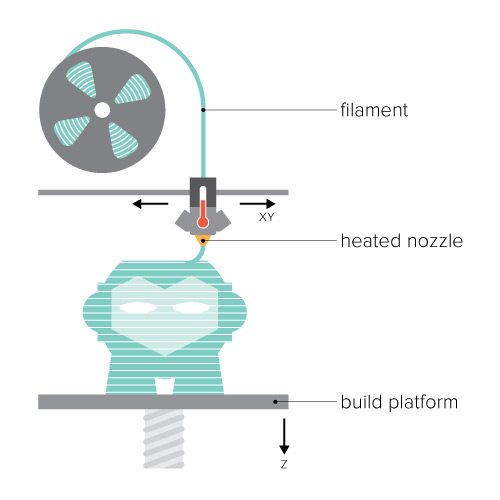
\includegraphics[width=0.4\textwidth, height=\textheight,keepaspectratio]{fdm_3d}
    \caption{Processo di stampa FDM}
    \label{fig:fdm_3d}
	\end{center}
\vspace{-40pt}
\end{wrapfigure}
FDM printing, also known as \emph{Fused Filament Fabrication} (FFF), consists of the deposition of a thermoplastic polymer, which is extruded through a thermoregulable nozzle on a plane, layer by layer until forming the three-dimensional model. This type of technology adapts to various low viscosity materials and thermoplastic materials, is inexpensive and relatively fast. The accuracy depends on the specifications of the printer, reaching up to a few tens of microns.
\pagebreak
\subsection{Stereolitografia (SLA)}
\begin{wrapfigure} {R} {0.37\textwidth}
\vspace{-40pt}
	\begin{center}
	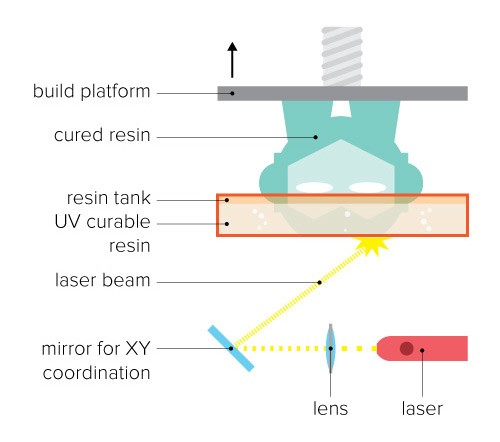
\includegraphics[width=0.37\textwidth, height=\textheight,keepaspectratio]{sla_3d}
    \caption{Processo di stampa SLA}
    \label{fig:sla_3d}
    \end{center}
\vspace{-40pt}
\end{wrapfigure}
Stereolithography was the first additive manufacturing technique to be patented in 1984 by \emph{Chuck Hull} \parencite{Reference124}. This technology uses a laser beam to locally polymerise the resin contained on the print layer, layer by layer. This type of printing is very precise and allows you to print various types of resins with different properties. In the dental field there are calcinable resins, resins for prostheses, for provisionals, for surgical guides and others.

\subsection{Digital Light Processing (DLP)}
\begin{wrapfigure} {R} {0.37\textwidth}
\vspace{-40pt}
	\begin{center}
	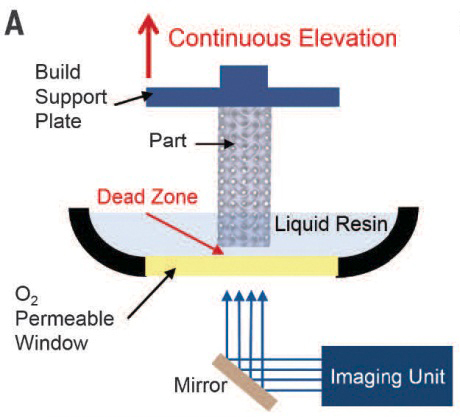
\includegraphics[width=0.37\textwidth, height=\textheight,keepaspectratio]{clip}
    \caption{Processo di stampa CLIP}
    \label{fig:clip}
    \end{center}
\vspace{-20pt}
\end{wrapfigure}
DLP printing also uses resin polymerization layer by layer, but instead of a laser such as SLA, it uses \emph{Digital Micromirror Device} (DMD, the same technology as projectors) to create a polymerization mask that it polymerizes the entire layer at once. This technique is very fast in producing objects. The print resolution depends on the resolution of the projected light beam, but in general it is very close to that of SLA. A recent evolution of DLP printing is the CLIP \parencite{Reference121}, \parencite{Reference122}, which allows very fast production of high-resolution structures. The CLIP technology was developed by the company Carbon Inc. \parencite{Reference123}.

\subsection{Selective Laser Sintering (SLS)}
\begin{wrapfigure} {R} {0.40\textwidth}
\vspace{-30pt}
	\begin{center}
	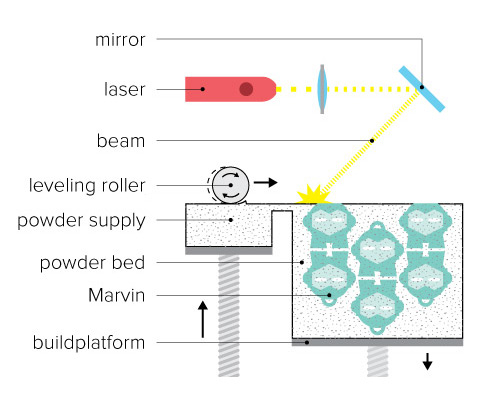
\includegraphics[width=0.40\textwidth, height=\textheight,keepaspectratio]{sls-technology}
    \caption{Processo di stampa SLS}
    \label{fig:sls-technology}
    \end{center}
\vspace{-40pt}
\end{wrapfigure}
SLS printers use a laser to sinter particles of polymers, metals and ceramics. The resolution is in the order of a few tens of micrometers. This technology finds various implications in the dental field, because it allows both to print polymers, then surgical guides and models, and to print ceramics and metals, with immediate possibilities of use in the prosthetic, implantological and surgical fields.
\newpage
\subsection{Material jetting (InkJet - PolyJet)}
\begin{wrapfigure} {R} {0.5\textwidth}
\vspace{-20pt}
	\begin{center}
	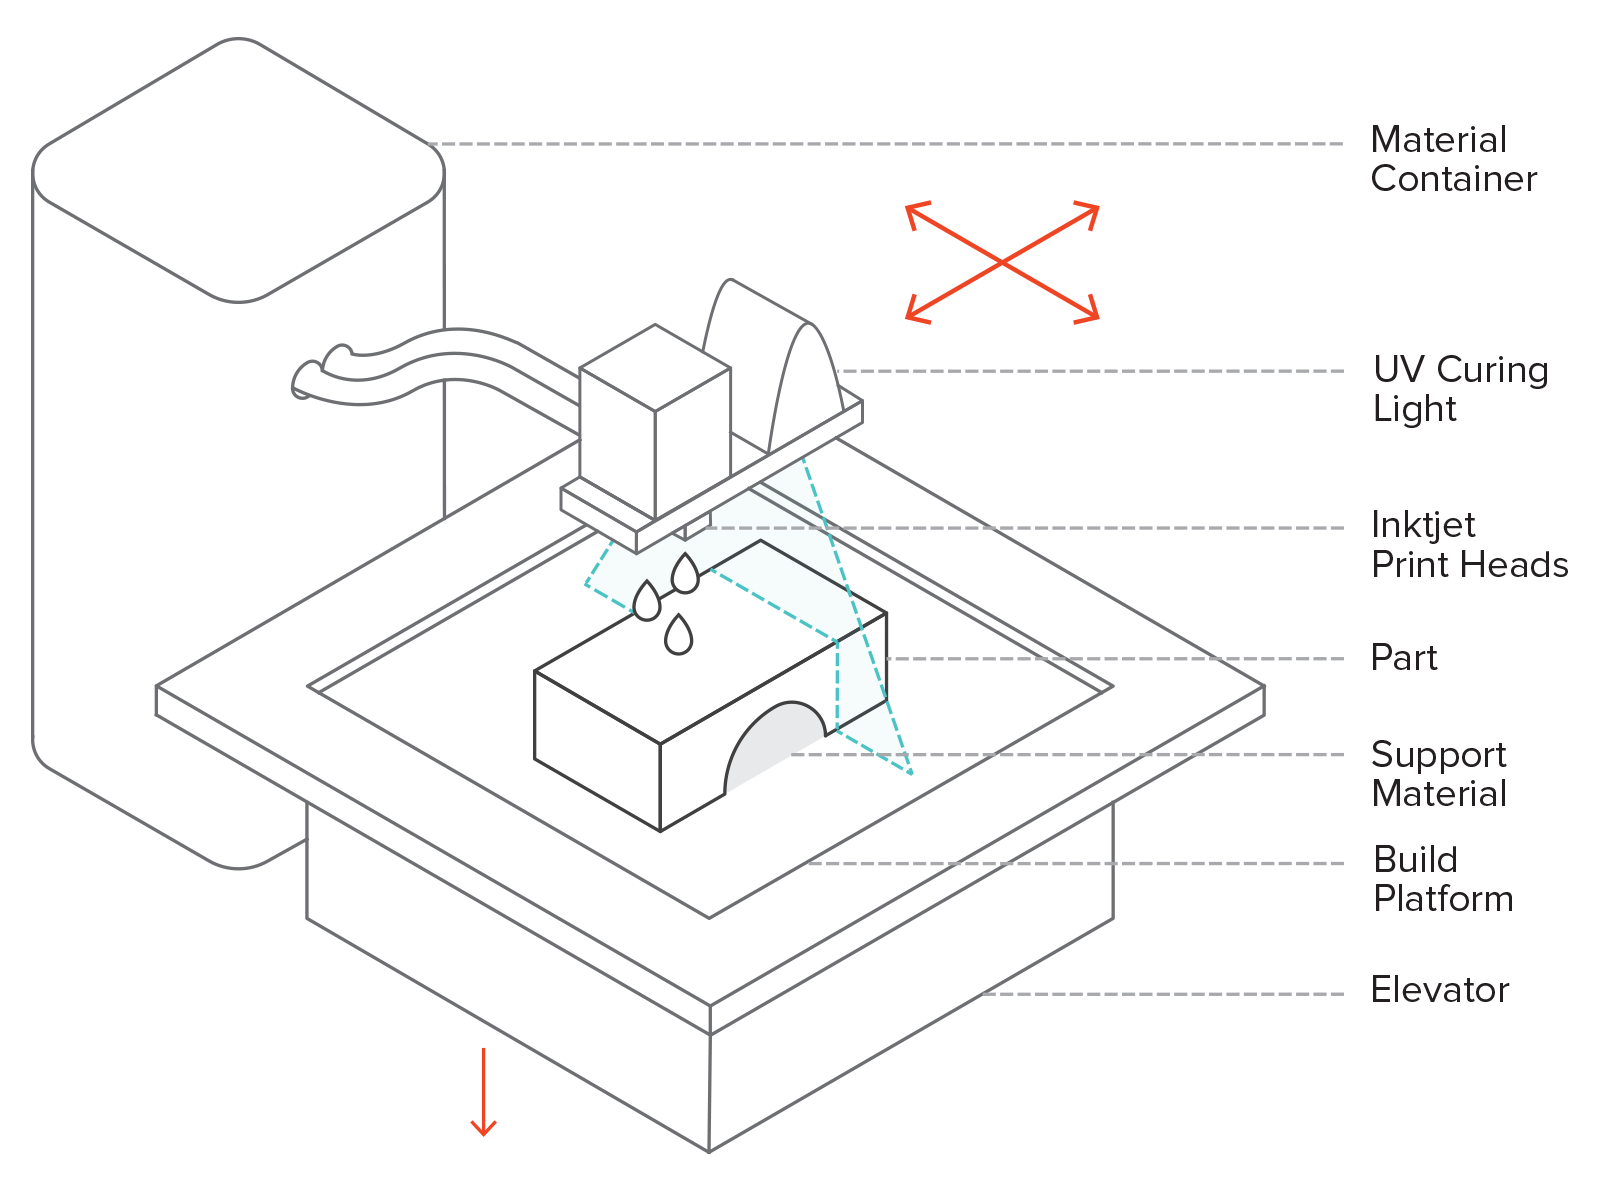
\includegraphics[width=0.5\textwidth, height=\textheight,keepaspectratio]{3-mj-schematic}
    \caption{Processo di stampa \emph{Material Jetting}}
    \label{fig:3-mj-schematic}
    \end{center}
\vspace{-20pt}
\end{wrapfigure}
The Material-jet print uses a printing head that moves on the printing surface depositing the material, which is then light-cured by a UV light, in a process very similar to 2D printing.
There are many print materials that can be printed simultaneously; this makes it possible to print objects with non-uniform mechanical characteristics, where for example there are both rigid and elastic areas. In addition to printing multiple materials at the same time allows you to print objects with a wide variety of colors. Printing is also very precise, because the layer of material deposited at each passage is very thin (in the order of \SI{20}{\micro\metre}).

\section{Starting the Print}
The Fused Deposition Modeling print process on a Cartesian printer is discussed here. \\
After obtaining the file in G-code from the slicing software, this file can be sent to the printer for printing. Depending on the capabilities offered by the printer's electronic control board, the G-code can be submitted to the printer in various ways.


\subsection{Printing via USB}
It consists of connecting the printer motherboard to the PC via a USB cable.
It has the advantage of being a fast method and allows the control of the printer from the graphic interface of the software installed on the PC \parencite{Reference2}. \\
A big disadvantage is the fact that the PC must necessarily be turned on throughout the printing process, and that any system crashes can stop printing suddenly and with little chance of recovery.

\subsection{Printing via SD Card}
Most of the motherboards for 3D printers currently on the market allow you to insert a microSD card, from which you can print the G-code files previously loaded on the card. \\
Printing from SD is very advantageous because it does not require the use of a PC during printing.
Many motherboards also allow you to load the G-code file on the microSD without removing it from the printer, simply by connecting the motherboard to the PC via USB to perform the transfer of the G-code on the microSD.
Printing from a memory card thus makes it possible to have a stand-alone 3D printer, which reduces the risk of printing failure due to problems that may occur to the PC during that phase.

\subsection{Printing via web interface}
More advanced motherboards, such as open-source \emph{Duet3D} \parencite{Reference3}, have the ability to connect to the Internet and allow printer control through the browser. This type of control greatly increases the flexibility of the printer, which can also be monitored while you are away from the printing place.
The web interface allows you to remotely control even more than one printer, provided that these are equipped with cards with web connectivity. This is extremely useful when multiple printers must be managed and monitored at the same time, as can happen in the educational field or in the industrial sector. Remote monitoring can also be performed by connecting a video camera to this card, which allows real-time video monitoring, saving the videos for later analysis or for the next projection for educational purposes.

\section{Calibration}
The calibration process varies depending on the printer model. The most advanced printers perform the calibration in an automated way, and require only a few checks by the operator. Cheaper or do-it-yourself printers can instead provide several steps where operator intervention is required. \\
The calibration must certainly be done before the first use, in order to have a reliable, precise and constant performance printer. The \parencite{Reference4} process consists of calibrating:

\begin{itemize}
\item Step by mm on the X, Y, Z and E axes (extruder)
\item Print bed level
\end{itemize}

\subsection{Step by millimeter}
To calibrate the steps for mm on the axes, you need to know some parameters of the printer components:

\begin{itemize}
\item \emph{\textbf{Angle per step}}: is the rotation that makes the axis for each step, measured in degrees. Generally corresponding to 1.8 / step (equal to 200 step / revolution) or 0.9 / step (equal to 400 step / revolution)
\item \emph{\textbf{Microstep}}: it depends on the interpolation capacity of the drivers that control the stepper motor on the motherboard. \parencite{Reference5}, \parencite{Reference6}. The microstep consists in sending low power pulses to the motor, to make it perform fractions of steps. This theoretically increases the print resolution, but as the interpolation increases, the torque decreases, so the motor may not have enough energy to perform the movement. This means that the fraction of rotation will not be performed until the number of pulses necessary to give sufficient torque to the motion is accumulated.
\item For axes with belt drive and pulleys (generally X and Y):

\begin{itemize}
\item Belt pitch in mm
\item Number of teeth of the pulley
\item steps / mm = (step / rev * microstep) / (belt pitch in mm * number of teeth of the pulley)
\end{itemize}

\item For axes with screw transmission (generally Z) \parencite{Reference51}:

\begin{itemize}
\item Screw pitch in mm
\item steps / mm = (step / rev * microstep) / screw pitch
\end{itemize}

\item For the extruder:

\begin {itemize}
\item step / mm = (step / rev * microstep) * / (diameter of the extrusion gear * pi)
\item With reduction (\emph{wade extruder}): step / mm = (step / rev * microstep) * (n large pulley teeth / small pulley teeth) / (extrusion gear diameter * pi)
\end{itemize}

\end{itemize}
	

\subsection{Leveling of the Press Bed}
Adjusting the printing plane should be as horizontal as possible to have an optimal surface on which to deposit the printing material. The plane must be orthogonal to the Z-beam and parallel to the X and Y axes. This arrangement allows to have an optimal deposition of the first layer, which is fundamental to guarantee the correct geometry of the printed object, as well as favoring its adhesion to the bed . \\
The top can be adjusted manually, adjusting the height through screws, or in an automated manner. Automated leveling (\emph{Auto Bed Leveling}) is performed with the aid of one or more sensors that allow you to define the position in the space of the couch. Any inclination of the table is then compensated by the motion of the extruder on the axis Z \parencite{Reference7}, \parencite{Reference8}. The leveling of the bed must be carried out with the extruder and printing plate at the working temperature to take into account the deformation of the components at high temperatures. \\
The auto bed leveling is performed with the G29 command. At the end of the bed survey, the machine reports a matrix with the data relating to the operation just carried out. This data can be used to get a better understanding of the bed's inclination, and can help us adjust the bed and choose the best area to print a model.
Data can be plotted thanks to scripts on websites \parencite{Reference9}. The Duet3D card also allows the display of the print plan \emph{heatmap} directly from the web \parencite{Reference10} interface.

\section{Print}
At the end of the printer's heating and leveling procedures, printing begins. The use of brim is recommended for priming the extruder and increasing the adhesion of the object.
To obtain a fine adjustment of the printing of the first layer, there is some firmware (Marlin, RepRap firmware) the \emph{BabyStep} option (in Marlin \emph{Babystepping}) that gives the possibility, during printing, to send axis movements to adjust its position. The Babystep is very useful in the printing of the first layer, because it gives us the possibility to precisely adjust the position of the nozzle with respect to the printing plane, facilitating the creation of a first layer uniform and well spread on the plane.
After any adjustment with Babystep has been carried out, printing continues until finished.
